\section{Architecture Definition}

This section will outline the system's initial state before introducing any eID solution. This outline will set a baseline to test accurately and validate the research findings.

For better clarity with terminology, the company wishing to integrate eID authentication is a physical exercise data tracking enterprise, \textbf{WorkAuth}. They are the relying party with respect to the eID solution providers. For a list of other abbreviations, see \hyperref[appendix:glossary]{Appendix I}

\subsection{System Architecture}

This section will focus on the technological architecture surrounding the integration; we will explain the business requirements for the system to illustrate the intended use case.

\subsubsection{System Overview}

\begin{figure}
  \centering
  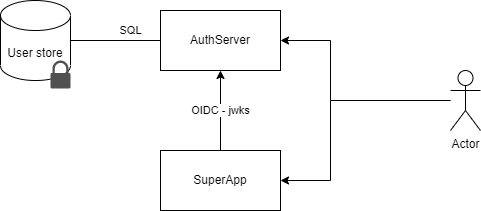
\includegraphics[scale=0.65]{architecture/initial.png}
  \caption{Initial system architecture}
  \label{fig:sys-highlevel}
\end{figure}

\paragraph{Initial state}

Figure \ref{fig:sys-highlevel} shows us a high-level overview of a system where we are trying to integrate eID authentication. This system consists of the following components:

\begin{enumerate}
  \item AuthServer. The company's authentication server. Acts as a central authority for identity. This server issues OIDC id tokens containing user ID numbers, roles, and claims. It is the primary access control mechanism in the company.
  \item SuperApp. A resource server with access control enabled. It uses OIDC id tokens issued by AuthServer and verifies them using public-key cryptography. It contains the data the company is trying to protect with stricter access control.
  \item User store. A data store containing user log-in information - usernames, password hashes, other Personally Identifiable Information (PII).
  \item Actor. A person accessing the resources in the system. Typically can be anyone, including computers; however, only natural persons holding an eID will be considered in our thesis's scope.
\end{enumerate}

\paragraph{Desired state}

The company WorkAuth wishes to implement eID authentication. Since the authentication is not done locally but is delegated to some remote service or device, the protocol can be treated as an external federated log-in. Application development frameworks such as ASP.NET Identity have helpful tools to handle external identity providers.

With the inclusion of an external eID provider, we can compose the new system architecture to be akin to Figure \ref{fig:sys-highlevel-witheid}. In this figure we can see two significant additions:

\begin{figure}
  \centering
  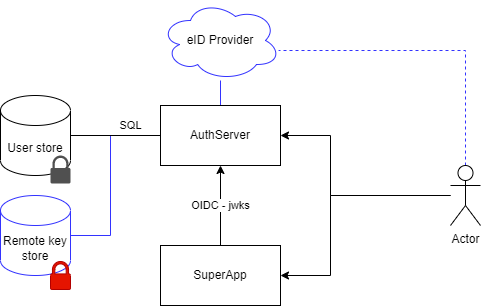
\includegraphics[scale=0.65]{architecture/witheid.png}
  \caption{System architecture after the inclusion of an eID provider}
  \label{fig:sys-highlevel-witheid}
\end{figure}

\begin{enumerate}
  \item {eID provider}. It is WorkAuth's gateway to obtain someone's eID. It can be any eID source such as Dokobit, TARA, Smart-ID, or an ID card.
  \item {Remote key store}. Storage for unique identifiers provided by the eID provider. These keys are the person identifying information.
\end{enumerate}

The primary purpose of the remote key store is to link the user ID used in the internal system with the unique identifier given by the eID provider. Because the unique identifier can change or the same physical person can have multiple eIDs \cite{eidas-saml}, companies should foresee cases where numerous eIDs could map to a single internal ID.

In the diagram (Figure \ref{fig:sys-highlevel-witheid}), the key store has a red lock next to its icon. The data stored there may be subject to more strict privacy regulations in some countries than others. Companies must ensure sufficiently strict access control for this part of the infrastructure to satisfy the legal requirements.

\paragraph{Final state}

The end goal for the scope of this thesis is to implement three eID providers into the architecture. For regular companies, it would make sense to implement multiple only if they would like to get more coverage. Additionally, they could register non eID providers, such as Google or Microsoft social log-ins; however, we will not cover this in the thesis. The final high-level overview of the system can be seen in Figure \ref{fig:sys-highlevel-final}.

\begin{figure}
  \centering
  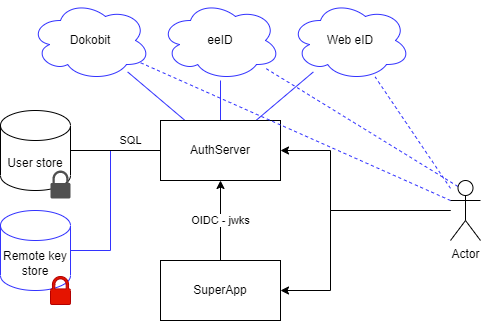
\includegraphics[scale=0.65]{architecture/final.png}
  \caption{System architecture after the inclusion of all eID providers in scope}
  \label{fig:sys-highlevel-final}
\end{figure}

The link to the repository containing the source code of the final system can be found in \hyperref[appendix:source]{Appendix III}.

\subsubsection{Process Overview}

The desired system must satisfy two business use cases.

The first one (see Figure \ref{fig:sysprocess-a}) is concerned about accessing a protected resource with a token issued by the AuthServer. This use case is part of the base state of the system and validates that the baseline implementation is correct.

The second use case (see Figure \ref{fig:sysprocess-b}) is also concerned with accessing a protected resource. This time it is intended to limit access to only those who authenticate with a higher level of assurance, like an eID solution. This process validates the successful implementation of eID authentication and access control.

\begin{figure}
  \centering
  {\small{
      \begin{sequencediagram}
        \newthread{A}{Actor}{}
        \newinst[3]{B}{AuthServer}{}
        \newinst[3]{C}{SuperApp}{}

        \begin{call}{A}{accessProtected()}{C}{401 Unauthorized}\end{call}

        \begin{call}{A}{authWithPassword()}{B}{Auth token}\end{call}
        \begin{call}{A}{accessProtected()}{C}{Data}\end{call}
        \begin{call}{A}{accessReallyProtected()}{C}{403 Forbidden}\end{call}
      \end{sequencediagram}
    }}
  \caption{System behavior when authenticated with a username + password scheme}
  \label{fig:sysprocess-a}
\end{figure}

\begin{figure}
  \centering
  {\small{
      \begin{sequencediagram}
        \newthread{A}{Actor}{}
        \newinst[3]{B}{AuthServer}{}
        \newinst[3]{C}{SuperApp}{}

        \begin{call}{A}{accessProtected()}{C}{401 Unauthorized}\end{call}

        \begin{call}{A}{authWithEid()}{B}{Auth token}\end{call}
        \begin{call}{A}{accessProtected()}{C}{Data}\end{call}
        \begin{call}{A}{accessReallyProtected()}{C}{Very Secret Data}\end{call}
      \end{sequencediagram}
    }}
  \caption{System behavior when authenticated with an eID scheme}
  \label{fig:sysprocess-b}
\end{figure}

\subsubsection{Linking eID to Internal User Accounts}

There will be a need to uniquely link an identity to an internal account in the company SSO server. The security requirement, in this case, is not to allow other users to access the same account. For this goal, companies must use one or more person-identifying properties.

Using Estonia's passport as an example, we see that it has the following identifiers: (issuer) country code, document number, surname, given name, personal code, citizenship, date of birth, document date of issue, expiry, and authority. In these cases, it is easy to use the {personal code} for identifying a person as it is unlikely to change - people change names, and documents expire. Document authority information and date of birth do not narrow it down nearly enough. The use of a personal number seems like an obvious choice.

Unfortunately, not all countries have personal numbers. If we look at Ireland's, another EU member state's, passport, we would be unable to find such a code. The lack of an id number shows one of the many challenges eID authentication adopters will face. If the data on the passport is all we would have, the next best unique identifier for linking users would be to use the document number. It is cumbersome and would require users to update the account with a new number when the document eventually expires and is replaced. Still, no other option satisfies the security condition requiring an eID to link only to the correct user as effectively as this one.

If we look at the eIDAS node network, its architecture does not have strong opinions on how an ID should look, as long as it has a country code and a unique code from the country. Each country must provide an identifier, even if the government doesn't have assigned a code to a person \cite{eidas-saml}. How countries achieve uniqueness is not of the network's concern.

The eIDAS node architecture solves another issue of what to do if a person's identifier changes. A unique identifier remains "unchanged for the lifetime of the account" \cite{eidas-saml}. If an identifier were to change when "the user's digital identity is replaced or repaired," relying parties should treat the newly obtained identifier as a completely new identity.

\paragraph{eIDAS Unique Identifier Structure} In eIDAS SAML Attribute Profile, an identifier code is defined as:
\begin{enumerate}
  \item The first part is the Nationality Code of the identifier. Value is an ISO 3166-1 alpha-2 code, followed by a slash ("/")).
  \item The second part is the Nationality Code of the destination country or international organization. Value is an ISO 3166-1 alpha-2 code, followed by a slash ("/").
  \item The third part is a combination of readable characters. This sequence of characters uniquely identifies the identity asserted in the country of origin but does not necessarily reveal any discernible correspondence with the subject's actual identifier (for example, username, fiscal number, etc.).
\end{enumerate}

Example: ES/AT/02635542Y (Spanish eID Number for an Austrian SP).

\paragraph{Summary} Using the eIDAS Unique Identifier structure as a base, we can see that it is enough to uniquely identify a digital identity in eIDAS with the country of origin, country of destination, and a set of characters to identify that person in the origin country. The destination country will always be the same in our company's case. To uniquely identify a person, we will only need its origin country and a unique identifier a member state must provide.

As a result, our chosen identifier structure will be of the following: "{\{ISO 3166-1 alpha-2\}}/{\{Code provided by country\}}". Unique identifier examples: EE/38001085718, LT/49003111045, SE/870314-2391.

\subsubsection{Privacy Policy}

A company wishing to implement eID authentication will have to deal with personal information as described by GDPR \cite{eulaw-gdpr}. Before going live with an eID solution, they must conduct a legal audit for compliance.

A privacy policy is a legal document and is outside of the scope of a technical implementation thesis. However, it is still important to understand the basics. For this goal, two privacy policies will be analyzed: Web eID \cite{legal-webeid-privacypolicy} and Dokobit \cite{legal-dokobit-privacypolicy}.

From the cursory analysis of the two policies, there are three fundamental aspects any company needs to address: what data is processed, with whom the company shares the data, and what is the retention policy. An actual privacy policy varies drastically from case to case.

Based on the privacy policies of Web eID and Dokobit, we constructed a rudimentary privacy policy for the use of the test application environment. The thesis \hyperref[appendix:privacy]{Appendix IV} contains a copy of the final text.

\subsection{Weaknesses in the Architecture}

When analyzing the weaknesses of WorkAuth's internal systems, it is good to understand their cause. Some vulnerabilities can appear due to existing issues, faulty implementation, or deeply rooted issues in the architecture itself. In this chapter, we will address these categories.

\paragraph{eID provider dependant weaknesses}

These threats come from one common issue: trusting an eID service provider when a relying party should not have. There are four primary causes:

\begin{enumerate}
  \item relying party trusts data from an insecure channel;
  \item relying party does not perform the necessary validation mandated by the protocol;
  \item inherent weakness in the architecture of the used data transfer protocol;
  \item eID provider itself gets compromised;
\end{enumerate}

The thesis will address these points on a case-by-case basis for each eID provider in the study. We will address each of these points in the case studies' respective chapters.

\paragraph{Local weaknesses}

In Figure \ref{fig:sys-highlevel-witheid}, four system components do not interact with an eID solution: AuthServer, SuperApp, application store, user store, and remote key store. We can identify weaknesses in those parts and analyze each of them through the lens of CIA (confidentiality, integrity, availability) security analysis.

\subsubsection{SuperApp}

\paragraph{[CI] Users can see and or edit data normally forbidden to access} This issue is caused by one of the following:

\begin{enumerate}
  \item access control measures are disabled on a specific resource;
  \item OIDC token validation is disabled or misconfigured;
\end{enumerate}

The first cause has a trivial fix - developers have likely forgotten to enable the data access protection on the API endpoint.

In the case of the second cause, some corners were likely to be cut in the ID token validation process. When validating a token, the process has to match the one described in the OIDC spec \cite{oidc} exactly. This process consists of three major parts:

\begin{enumerate}
  \item check if the token's crypto algorithm is as expected;
  \item validate token signature;
  \item validate claims - issuer, audience, timestamp, nonce;
\end{enumerate}

Developers usually need not worry about this vulnerability, as most frameworks have adopted the OpenID Connect protocol or have well-maintained libraries.

\paragraph{[A] Service becomes unavailable} This threat is caused by one of the following:

\begin{enumerate}
  \item server is offline or overloaded;
  \item OIDC token validation is misconfigured to have an incorrect authority;
\end{enumerate}

The first case is a common availability issue, meaning the server is suffering a denial of service attack. We will not cover the mitigation of this form of availability threat in the scope of the thesis.

A likely cause for the second part of this issue is the manually configured OIDC properties on the relying party. If possible, developers should never configure the properties manually and use the well-known metadata endpoint instead. A metadata endpoint usually looks like this - \url{https://auth.mycompany.org/.well-known/openid-configuration}.

\subsubsection{AuthServer}

All of the points that apply to SuperApp also apply to AuthServer. However, there is a critical use case that is worth mentioning explicitly.

\paragraph{[CI] Users can see used eID schemes and add new ones with unsafe log-in}

As per usability requirements, users must be able to assign multiple identity providers to their accounts. When adding a new external scheme, the currently logged-in user must have the same privilege level as the scheme they are trying to add. This countermeasure is in place if an adversary gains access to their account; they wouldn't be able to elevate their privileges by adding their eID scheme and signing in with it.

With this requirement in place, registration with an email and password becomes less valuable, as those accounts could never add an eID afterward. Companies can enact an exception to this security requirement for the first eID scheme a user would add. However, a better solution would be to have a company policy to verify the user's first added eID manually.

In short, if a person logs in with a low level of assurance, they should not be able to add a higher level of assurance authentication scheme to the same account as that would artificially elevate their account trust.

\subsubsection{Data Stores}

All three data stores have the exact issues between them. For the sake of brevity, we will group them under the umbrella of \textit{data store}.

\paragraph{[CI] Users have a less secure way of accessing the data store}

The system is as secure as its weakest link. If users or developers have direct access to the database while bypassing the eID authentication check, the security and assurance guarantees are worthless.

If there are alternative ways of accessing the database, companies must implement proper access rules that would be as secure as the one's eIDs provide. How companies can achieve that depends on what data storage options they use. The best option would be to completely close down external or internal access to the data stores.

\paragraph{[CI] Man-in-the-middle attacks} While uncommon, some data stores are vulnerable to MitM attacks \cite{sql-server-auth-mitm}. Although the best course of action would be to move the data storage server away from the internet and make it accessible only on the local network or via a VPN. However, in cases where an attacker has access to the internal network, even that is not enough. For maximum security, companies must implement the recommended MitM prevention techniques \cite{sql-server-enable-tls}.

\paragraph{[A] Data is destroyed or lost}

Ransomware attacks and accidental database corruptions can happen, so offline remote backups are a must.

An interesting issue arises when companies should treat backups to the same security standards as live databases. One approach to ensuring data integrity and confidentiality would be encryption; keys should only be available after authenticating with an eID scheme. One equally secure alternative would be to use something like the encryption and decryption functionality of Estonia's ID cards.